\documentclass[11pt,a4paper]{article}

\usepackage[polish]{babel}
\usepackage[utf8]{inputenc}
\usepackage{polski}
\usepackage[T1]{fontenc}
\usepackage{indentfirst}
\usepackage{wrapfig}    % for wrapping figures, tables

\frenchspacing

%\usepackage{amsmath}
\usepackage{physics}
%\usepackage{bm}
\usepackage{gensymb}
%\usepackage{hepnames}
\usepackage{epsfig}
\usepackage{graphics}
\usepackage[shortlabels]{enumitem}
%\usepackage{xspace}
%\xspaceaddexceptions{[]\{\}}

%
%
%fixpagesize
\pagestyle{empty}
\addtolength{\textwidth}{6cm}
\addtolength{\textheight}{4cm}
\addtolength{\evensidemargin}{-3cm}
\addtolength{\oddsidemargin}{-3cm}
\addtolength{\topmargin}{-2cm}
\parindent=0cm

%
%
%small distance in list/item/enum for enumitem package
\setlist[itemize,enumerate]{topsep=0em}
\setlist{noitemsep}


% definition of inexact differential symbol:
\newcommand{\dbar} {\ensuremath{\,\mathchar'26\mkern-12mu d}}

%print zadanie #
\newcounter{zadanie}\newcommand{\zadanie}[1][]{\addtocounter{zadanie}{1} ~\\  {\bf \emph{Zadanie \arabic{zadanie} #1 }} \\}
\newcounter{zaddom}\newcommand{\zaddom}[1][]{\addtocounter{zaddom}{1} ~\\  {\bf \emph{Zadanie domowe \arabic{zaddom} #1 }} \\}
%\renewcommand{\zadanie}[1][]{\pagebreak  ~\\  {\bf \emph{Zadanie }} \\} \addtolength{\topmargin}{-2cm}


%
%%%%%%%%%%%%%%%%%%%%%%%%%%%%%%%%%%%%%%%%%%%%%%%%%%%%%%
% Changes figure placing algorithm
\renewcommand{\topfraction}{1}       % maximal fraction of a page allowed for figures
\renewcommand{\textfraction}{0.15}   % minimal number of text for figure-text shared pages
\renewcommand{\floatpagefraction}{0.95} % if two above does not help, this could do the job
                                        % must be: floatpagefraction < topfraction !!!!
%
\renewcommand{\textfraction}{0} % minimum fraction of page, which must be
                                % devoted to text
\renewcommand{\topfraction}{1}  % maximum fraction at top, which can be
                                % occupied whit floats
\setcounter{totalnumber}{400}   % increase the number of floats for one page
\setcounter{topnumber}{200}     % at all/top/bottom.
\setcounter{bottomnumber}{200}  %


\begin{document}           % End of preamble and beginning of text.
\begin{centering}

\vspace*{-1cm}

\bf{\Large{Termodynamika z elementami fizyki statystycznej}}\\
Tydzień 14 (8 czerwca 2023)\\[5mm]
napięcie powierzchniowe, transport ciepła\\
\end{centering} 

\vspace*{0mm}
\zadanie
Zakładając, że energia potencjalna związana z napięciem powierzchniowym jednostronnej błony cieczy jest
równa $E_p = \sigma \cdot S$, gdzie $S$ – powierzchnia, $\sigma$ – współczynnik napięcia
powierzchniowego, policzyć energię błony rozpiętej na długich prętach rozmieszczonych
w narożach kwadratu, jeśli:\\[1mm]
\hspace*{10ex} a) błona tworzy kształt:
\hspace*{20ex} b) błona tworzy kształt: \\
\hspace*{13ex}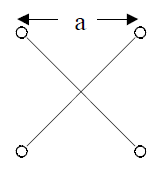
\includegraphics[width=22mm]{blona1.png}
\hspace*{32ex}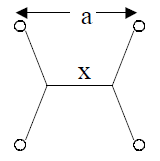
\includegraphics[width=22mm]{blona2.png}
\\
W którym przypadku energia jest mniejsza? Jakiej wartości $x$ odpowiadać będzie minimum energii?

\vspace{0.2cm}
\textbf{Rozwiązanie:}\\
W pierwszym przypadku błona rozpięta jest na dwóch prostokątach o wymiarach $ l \times a\sqrt{2}$. Wobec tego,
\begin{align*}
E_{p}^{(a)}= 2 \cdot 2 \sqrt{2}\sigma a l = 4 \sqrt{2}\sigma a l,
\end{align*}
gdzie uwzględniliśmy fakt, że obie błony mają dwie warstwy.

W podpunkcie b) mamy łącznie pięć prostokątów, cztery z nich mają wymiary $ l \times d$, gdzie $ d= \sqrt{\left(\frac{a}{2} \right)^2 + \left(\frac{a-x}{2} \right)^2  }$, a jeden z nich to prostokąt o wymiarach $l \times x$. W tym przypadku otrzymujemy, 
\begin{align}
E_p^{(b)} =  2 \cdot 4 \sigma l  \sqrt{\left(\frac{a}{2} \right)^2 + \left(\frac{a-x}{2} \right)^2}  + 2 \sigma l x= 2 \sigma l \left( 4 \sqrt{\left(\frac{a}{2} \right)^2 + \left(\frac{a-x}{2} \right)^2}  + x \right).
\end{align}
Minimum energii wyznaczamy z warunku:
\begin{align}
\left. \frac{{\rm d} E_p^{(b)}}{{\rm d} x} = 0 , \quad \frac{{\rm d^2} E_p^{(b)}}{{\rm d} x^2} \right\lvert_{x=x_{\rm min}}  > 0. 
\end{align}
\begin{align}
\frac{x-a}{\sqrt{\left(\frac{a}{2} \right)^2 + \left(\frac{a-x}{2} \right)^2} } + 1=0 \implies x_{\rm min} = \left( 1 - \frac{\sqrt{3}}{3}\right)a. 
\end{align}
Wyznaczmy wartość $E_p^{(b)}(x)$ w $x=x_{\rm min}  $:
\begin{align}
E_p^{(b)}(x_{\rm min}) = \frac{2\sigma l }{3}\left(  4 \sqrt{3} a + (3 -\sqrt{3})a\right) =2 \sigma l a (1 + \sqrt{3}  ) < E_p^{(a)}
\end{align}
Porównując energię potencjalne błonek w obu przypadkach otrzymujemy:
\begin{align}
E_p^{(a)} = E_p^{(b)} \Leftrightarrow x_1=0 \lor x_2 = \frac{4}{3}a \left(2 - \sqrt{2} \right), 
\end{align}
zatem w przypadku gdy $x_1\leq x \leq x_2$,  $E_p^{(a)}> E_p^{(b)}$, a w przedziale $x_2 \leq  x$,  $E_p^{(b)}> E_p^{(a)}$.

%%%%%%%%%%%%%%%%%%%%%%%%%%%%%%%%%
\newpage
%%%%%%%%%%%%%%%%%%%%%%%%%%%%%%%%%

\zadanie
Policzyć ciśnienie panujące wewnątrz bańki mydlanej o promieniu $r$.
Ile wynosi to ciśnienie dla $r = 1$\,mm? Przyjąć napięcie powierzchniowe takie,
jak dla wody $\sigma = 0.073$\,N/m.\\[1mm]
{\em Wskazówka: Porównać pracę potrzebną na powiększenie promienia bańki o $dr$
ze zmianą energii błony bańki.}

\vspace{0.2cm}
\textbf{Rozwiązanie:} 
Wyznaczmy na początek ciśnienie $p$ panujące wewnątrz kropli wody. Praca wykonywana przez kroplę wody przeciwko zewnętrznemu ciśnieniu $p_0$ przy zwiększaniu jej promienia o ${\rm d} R $ jest równa:
\begin{align}
{\rm \dbar W} =  (p-p_0) {\rm d}V = (p-p_0)d(\frac{4}{3}\pi R^{3}) =  (p-p_0) 4\pi R^2 {\rm d}R.
\end{align}
Praca ta jest równa energii powierzchniowej:
\begin{align}
{\rm d} E = \sigma {\rm d} A = \sigma d(4\pi R^{2}) = \sigma 8\pi R dR
\end{align}
Stąd;
\begin{align}
4\pi (p-p_0)R^2 {\rm d}R = \sigma 8 \pi R {\rm d}R \\
 p= p_0 + \frac{2 \sigma}{R}.
\end{align}
Bańka mydlana ma dwie powierzchnie powietrze-mydło (zewnętrzną i wewnętrzna). Przyjmijmy, dla uproszczenia, że mają one taką samą krzywiznę i promień. Wobec tego,
\begin{align}
p_f - p_0 = p- p_f = \frac{2 \sigma}{R} \\
p_f = p_0 +  \frac{2 \sigma}{R}, \quad p = p_f +  \frac{2 \sigma}{R}  \implies p = p_0 +  \frac{4 \sigma}{R},
\end{align}
gdzie $p_f$ jest ciśnieniem filmu woda+mydło.\\
%%%%%%%%%%%%%%%%%%%%%%%%%%%%%%%%%
\newpage
%%%%%%%%%%%%%%%%%%%%%%%%%%%%%%%%%

\zadanie
Szklaną kapilarę o wewnętrznym promieniu $R = 0.1$\,mm i długości $H = 20$\,cm wsunięto pionowo
do wody. Górny koniec rurki jest szczelnie zamknięty. Jaki odcinek $h$ kapilary należy zanurzyć,
aby poziom w rurce i na zewnątrz był jednakowy?
Przyjmij, że: ciśnienie powietrza $p_0 = 1020$\,hPa,
woda doskonale zwilża powierzchnię rurki (tzn. $\sigma=-\alpha$,
gdzie $\alpha$ jest współczynnikiem przylegania wody do szkła),
stała napięcia powierzchniowego wody $\sigma = 0.073$\,J/m$^2$,
oraz powietrze można traktować jako gaz doskonały.

\vspace{0.2cm}
\textbf{Rozwiązanie:} 
Rozważmy na początku wsuwanie otwartej kapilary. Z warunku równowagi ciśnienie na zewnątrz $p_0$ kapilary musi być równej ciśnieniu w jej wnętrzu, stąd:
\begin{align}
p_0 = \left( p_0 - \frac{F_\sigma}{S} \right) + \rho g h^{\prime},
\end{align}
gdzie $\frac{F_ \sigma}{S} = \frac{\sigma l}{S} $ jest ciśnieniem związanym z siła zwilżającą, a $h^{\prime}$ jest wysokością słupa wody w kapilarze.\\
Z powyższego warunku otrzymujemy:
\begin{align}
\frac{F_{\sigma}}{S} =  \rho g h^{\prime} \implies \rho g h^{\prime} = \frac{\sigma l}{S} = \frac{2 \pi\sigma r }{\pi r^2} = \frac{2 \sigma}{r}.
\end{align}
W przypadku wsuwania zamkniętej kapilary otrzymujemy analogicznie równanie:
\begin{align}
p_0 = \left( p^{\prime \prime} - \frac{F_{\sigma}}{S}\right) + \rho g h^{\prime \prime}.
\end{align}
Dodatkowo, z równania Clapeyrona mamy:
\begin{align}
p_0  H S = p^{\prime \prime} (H- h^{\prime \prime}) S,
\end{align}
gdzie $H$ jest długością kapilary nad poziomem wody.\\
Z powyższych równań otrzymujemy:
\begin{align}
p^{\prime \prime} &= p_0 \frac{H}{H-h^{\prime\prime}}\\
p_0 &= \left(p_0 \frac{H}{H-h^{\prime\prime}} - \frac{2 \sigma}{r} \right) + \rho g h^{\prime \prime} \implies 
\rho g h^{\prime \prime} =  \frac{2 \sigma}{r} + p_0 \left(1 - \frac{H}{H-h^{\prime \prime}} \right) 
\end{align}
W rozważanym problemie poziomy wody wewnątrz i na zewnątrz kapilary mają być takie same. Odcinek $h$ wyznaczymy rozwiązując następujący układ równań:
\begin{align}
\begin{cases}
p^{\prime \prime \prime}- \frac{F_{\sigma}}{S} + \rho g h =  p_0 + \rho g h \\
p^{\prime \prime \prime}(H-h) S = p_0 H S.
\end{cases}
\end{align} 
Po prostych przekształceniach otrzymujemy:
\begin{align}
h = \frac{H}{1 + \frac{p_0 r}{2 \sigma}}.
\end{align}

%%%%%%%%%%%%%%%%%%%%%%%%%%%%%%%%%
\newpage
%%%%%%%%%%%%%%%%%%%%%%%%%%%%%%%%%

\zadanie
Rozwiązać jednowymiarowe równanie transportu ciepła:
\[ \frac{\partial T}{\partial t} = \frac{\lambda}{\rho c}\cdot
                                   \frac{\partial^2 T}{\partial x^2} \]
metodą rozdzielania zmiennych, czyli zakładając, że rozwiązania
bazowe mają postać iloczynu:
\[ T(x,t) = X(x)\cdot{\displaystyle \tau}(t).\]

\vspace{0.2cm}
\textbf{Rozwiąznie:} 
Wstawiamy postulowanie rozwiązanie bazowe do równia transportu ciepła:
\begin{align}
X(x) \dot{\tau}(t) = \frac{\lambda}{\rho c} \tau(t) X^{\prime \prime}(x), 
\end{align}
a stąd,
\begin{align}
\frac{\dot{\tau}(t)}{\tau(t)}= \frac{\lambda}{\rho c} \frac{X''(x)}{X(x)}.
\end{align}
Lewa strona powyższego równania zależy wyłącznie od czasu, a prawa jest funkcją położenia x, oznacza to, że obie strony muszą być równe pewnej stałej:
\begin{align}
\frac{\rho c}{\lambda}  \frac{\dot{\tau}(t)}{\tau(t)}= \frac{X''(x)}{X(x)}= C^2.
\end{align}
Szukane rozwiązanie jest superpozycja:
\begin{align}
X_k = \exp{C_k x} + \exp{-C_k x}, \quad \tau_k = \exp{C_k^2 \lambda /(\rho c) t}.
\end{align} 
Ostatecznie, 
\begin{align}
T(x, t) = \sum_k \left( A_k \exp{C_k x} + B_k \exp{-C_k x} \right) \exp{C_k^2 \lambda /(\rho c) t} \label{eq:roz}
\end{align}

%%%%%%%%%%%%%%%%%%%%%%%%%%%%%%%%%
\newpage
%%%%%%%%%%%%%%%%%%%%%%%%%%%%%%%%%
 
\zadanie
Pręt styka się na obu końcach z ciałami o temperaturze $T_1$.
W chwili początkowej rozkład temperatury w pręcie dany jest funkcją:
\[ T(x,t=0) \,=\, T_1 + A \cos^3 \left(\frac{\pi x}{L}\right), \]
gdzie $-L/2 < x < L/2$.
Jak zależy od czasu rozkład temperatury w pręcie?\\[1mm]
{\em Wskazówka: Skorzystać z równości
~$\cos{\alpha} = {1\over 2} (e^{i\alpha}+e^{-i\alpha})$ i ze wskazówki z poprzedniego zadania.}

\vspace{0.2cm}
\textbf{Rozwiąznie:} 
Rozpisujemy funkcję $\cos{x}$:
\begin{align}
\cos{x} = \left( \frac{e^{i x} +  e^{-i x} }{2}\right)^3 = \frac{1}{8}\left(e^{3i x} + 3 e^{i x} + 3 e^{-i x} + e^{-3i x}\right)= \frac{1}{4} \cos{3x} + \frac{3}{4}\cos{x}.
\end{align}
Zatem warunek początkowy możemy przekształcić do postaci:
\begin{align}
T(x, t=0) = T_1 + \frac{A}{4} \cos{\frac{3 \pi x}{L}} + \frac{3A}{4} \cos{\frac{ \pi x}{L}}.
\end{align}
Korzystając z rozwiązania \eqref{eq:roz} znajdujemy:
\begin{align}
A_0 = \frac{T_1}{2}, B_0 = \frac{T_1}{2},  C_1 = 0 \\
A_1= \frac{A}{8}, B_1= \frac{A}{8}, C_k = \frac{i 3 \pi}{L}\\
A_2= \frac{3A}{8}, B_2= \frac{3A}{8}, C_k = \frac{i \pi}{L}\\
\end{align}
Po uproszczeniu otrzymujemy:
\begin{align}
T(x, t ) = T_1 + \frac{A}{4} \cos{\left( \frac{3 \pi}{L}x \right)} \exp{- \frac{9 \pi^2}{L^2}\frac{\lambda}{\rho c}t} + \frac{3}{4}A \cos{\left( \frac{ \pi}{L}x \right)} \exp{- \frac{\pi^2}{L^2}\frac{\lambda}{\rho c}t}.
\end{align}

%%%%%%%%%%%%%%%%%%%%%%%%%%%%%%%%%
\newpage
%%%%%%%%%%%%%%%%%%%%%%%%%%%%%%%%%

\zadanie
Znaleźć rozkład temperatury w gruncie w stanie ustalonym przy założeniu,
że grunt jest ośrodkiem jednorodnym o poziomej powierzchni oraz że
temperatura na powierzchni gruntu zmienia się zgodnie ze wzorem:
\[ T(x=0, y,z,t) \,=\, A \cos(\omega t) + T_\circ. \]

\vspace{0.2cm}
\textbf{Rozwiązanie:} W rozważanym problemie temperatura gruntu zależy wyłącznie od czasu i głębokości. Równanie transportu redukuje się do postaci przedstawionej w zadaniu 4. \\
Postulujemy, że szukane rozwiązanie jest postaci:
\begin{align}
T(t, x) =T_0 + A \exp{a x} \cos{(\omega t - kx)}.
\end{align}
Wobec tego:
\begin{align}
\dot{T} \equiv \frac{\partial T(t, x)}{\partial t} =- A \exp{\alpha x}\omega \sin{(\omega t - kx)},
\end{align}
\begin{align}
T^\prime \equiv \frac{\partial T(t, x)}{\partial x} = A \exp{\alpha x} \left(\alpha \cos{(\omega t - kx)} + k \sin{(\omega t - kx)}\right)
\end{align}
i 
\begin{align}
T^{\prime\prime} \equiv \frac{\partial^2 T(t, x)}{\partial x^2} = A \exp{\alpha x} \left(\alpha^2 \cos{(\omega t - kx)} + 2 \alpha k \sin{(\omega t - kx)}-  \alpha k^2 \cos{(\omega t - kx)}\right)
\end{align}
Porównując odpowiednie współczynniki przy funkcjach trygonometrycznych otrzymujemy:
\begin{align}
(\alpha^2 - k^2)\cos{(\omega t - kx)} = 0 \implies a= \pm k\\ 
2 \alpha k \sin{(\omega t - kx)} = - \omega \frac{\rho c}{\lambda} \sin{(\omega t - kx)} \implies a = \pm \sqrt{\frac{c \rho \omega}{2 \lambda}}.
\end{align}
Współrzędna x rośnie wgłąb ziemi, wobec tego współczynnik $a$ powinien być ujemny (fluktuacje temperatury powinny zanikać z głębokością). Ponieważ iloczyn $a k$ jest ujemny, $k$ musi być dodatnie.\\
Rozwiązanie przedstawia  falę sinusoidalną,  o eksponencjalnie zanikającej amplitudzie i o przesunięciu fazowym rosnącym liniowo wraz z głębokością. 
%%%%%%%%%%%%%%%%%%%%%%%%%%%
\newpage 
%%%%%%%%%%%%%%%%%%%%%%%%%%%
\zaddom
Po powierzchni wody pływa krążek aluminiowy o grubości
$d = 0.1\,$mm i promieniu $R = 1\,$cm.
Jaki kąt tworzy z poziomem powierzchnia wody przy brzegu krążka?
Gęstość aluminium $\rho = 2.7\,{\rm g/cm^3}$,
napięcie powierzchniowe wody $\sigma = 7.3\cdot 10^{-2}\,$N/m.
Krążek nie jest zwilżany przez wodę.


\zaddom
Na płaskiej powierzchni znajduje się kropla o objętości $V$.
Energia napięcia powierzchniowego cieczy jest równa $E_1 = \sigma \cdot S_1$.
Energia przylegania ciecz -- ciało stałe jest równa $E_2 = \alpha \cdot S_2$.
Założyć, że powierzchnia kropli będąca w kontakcie z powietrzem ($S_1$)
jest wycinkiem kuli o promieniu $R$, zaś powierzchnia kropli będąca
w kontakcie z ciałem stałym ($S_2$) jest kołowa. Przyjmij, że przy zmianach
kształtu objętość kropli pozostaje stała.
Wykazać, że energia układu jest najmniejsza, kiedy kąt przylegania
$\theta$ spełnia warunek: $\cos{\theta} = -\alpha/\sigma$.
Przyciąganie ziemskie pomijamy.


\zaddom
Rurka barometryczna o średnicy wewnętrznego przekroju $d = 4\,$mm wypełniona jest rtęcią i zanurzona otwartym
końcem w szerokim naczyniu z rtęcią. Różnica poziomów rtęci w rurce i naczyniu wynosi $\Delta h = 756\,$mm.
Jakie jest ciśnienie atmosferyczne, jeżeli wiadomo, że rtęć jest cieczą całkowicie niezwilżającą (tzn. kąt zwilżania $\theta = \pi$) dla szkła?
Gęstość rtęci $\rho = 13.56\,{\rm g/cm^3}$.
Współczynnik napięcia powierzchniowego $\sigma = 0.47\,$N/m.


\zaddom
Do cieczy w szerokim poziomym naczyniu włożono pionowo cienką rurkę o wewnętrznym promieniu równym $r$.
Współczynnik napięcia powierzchniowego cieczy jest równy $\sigma$,
współczynnik przylegania cieczy do ciała stałego jest równy $\alpha$.
\begin{enumerate}
\item Jakie jest położenie górnego poziomu cieczy wewnątrz rurki?
      Wynik przedyskutować w funkcji współczynnika $\alpha$.
\item Na jaką wysokość wzniesie się woda w rurce szklanej o promieniu $r = 1$\,mm
      na Ziemi i na Księżycu (6 razy mniejsze natężenie pola grawitacyjnego)?
      Zakładamy idealne zwilżanie szkła przez wodę (tj. $\theta = 0$,
      gdzie $\theta$ – kąt zwilżania,
      $\cos{\theta} = - \alpha/\sigma$); dla wody $\sigma = 7\cdot 10^{-2}$~N/m.
\item Jaka musiałaby być średnica rurki celulozowej, aby woda wzniosła się w niej na
      wysokość $h = 10$\,m? Zakładamy idealne zwilżanie rurki celulozowej przez wodę.
\end{enumerate}

\zaddom
Energia płynie od ciała o temperaturze $T_2 = 500\,$K do ciała o temperaturze
$T_1 = 300\,$K przez dwa „szeregowo” połączone pręty o tej samej długości i tym samym polu przekroju.
Jeden z prętów wykonany jest z miedzi ($\lambda_{Cu} = 400\,{\rm \frac{W}{m\cdot K}}$),
a drugi z żelaza ($\lambda_{Fe} = 50\,{\rm \frac{W}{m\cdot K}}$).
Jaka jest temperatura $T$ połączenia prętów?


\zaddom
Pręt styka się na obu końcach z ciałami o stałej temperaturze $T_1$.
W chwili początkowej rozkład temperatury w pręcie dany jest funkcją
$T(x,0) = T_1 + A\cdot \sin(x)+\frac{A}{2}\cdot \sin(2x)$, gdzie
$x\in [0, \pi]$. Jak zależy od czasu temperatura pręta?



% An example of figure placement:
%\begin{wrapfigure}[13]{r}{0.4\linewidth}\vspace{3mm}
%\resizebox{\linewidth}{!}{\includegraphics{NAZWA.png}}
%\end{wrapfigure}
%\zaddom

\end{document}
